% This is the LaTeX template file for homework for CSC549, Advanced Algorithm Design and Analysis.  When preparing homework solutions for this class, please use this template.
%
% This LaTeX template was created by the UC Berkeley EECS dept.
%
%

\documentclass[twoside]{article}
\setlength{\oddsidemargin}{0.25 in}
\setlength{\evensidemargin}{-0.25 in}
\setlength{\topmargin}{-0.6 in}
\setlength{\textwidth}{6.5 in}
\setlength{\textheight}{8.5 in}
\setlength{\headsep}{0.75 in}
\setlength{\parindent}{0 in}
\setlength{\parskip}{0.1 in}

%
% add packages if you need them here:
%

\usepackage{amsmath,amsfonts,graphicx}
\usepackage{algorithm,caption}
\usepackage[noend]{algpseudocode}
\usepackage{tikz}
%
% the following macro is used to generate the header.
%
\newcommand{\homework}[4]{
   \pagestyle{myheadings}
   \thispagestyle{plain}
   \newpage
   \setcounter{page}{1}
   \noindent
   \begin{center}
   \framebox{
      \vbox{\vspace{2mm}
    \hbox to 6.28in { {\bf CSC 349-07: Design and Analysis of Algorithms
		\hfill Winter 2023} }
       \vspace{4mm}
       \hbox to 6.28in { {\Large \hfill P vs NP:  March 7, 2023 \hfill} }
       \vspace{2mm}
       \hbox to 6.28in { {\it Instructor: Rodrigo Canaan \hfill Scribe: Ishaan Sathaye} }
      \vspace{2mm}}
   }
   \end{center}
}


% use these for theorems, lemmas, proofs, etc.
\newtheorem{theorem}{Theorem}
\newtheorem{lemma}[theorem]{Lemma}
\newtheorem{proposition}[theorem]{Proposition}
\newtheorem{claim}[theorem]{Claim}
\newtheorem{corollary}[theorem]{Corollary}
\newtheorem{definition}[theorem]{Definition}
\newtheorem{note}[theorem]{Note}
\newenvironment{proof}{{\bf Proof:}}{\hfill\rule{2mm}{2mm}}

% **** you may define additional macros here:
\algnewcommand\algorithmicinput{\textbf{Input:}}
\algnewcommand\INPUT{\item[\algorithmicinput]}

\algnewcommand\algorithmicoutput{\textbf{Output:}}
\algnewcommand\OUTPUT{\item[\algorithmicoutput]}

\begin{document}
\homework

\section{Announcements}

\begin{itemize}
    \item No new programming assignment
    \item Quiz 3 and other quizzes missed retake this Thursday (March 9, 2023)
    \item Look out for an activity next week
\end{itemize}

\section{Complexity}

\subsection{Big O}

{\em Big O time complexity does not care about multiplicative constants.} For example, consider
a matrix multiplication algorithm. Reading a contiguous chunk of memory would be faster 
than reading columns in another matrix. However, Big O does not care about this.

\subsection{Polynomial vs. Non-Polynomial}
Time complexities such as $O(n^2)$, $O(n^3)$, $O(2^n)$, $O(n!)$, and $O(n^n)$ are all polynomial time complexities
and bounded by a polynomial.

An example of a non-polynomial time complexity would be $O(2^{n})$, which is
significantly worse than something like $O(n^{100})$.

\section{NP}

\subsection[Decision Problems] {Decision Problems\footnote{We will be focusing more on these types of NP Problems}}

\begin{definition}
A problem for which any proposed solution can be quickly checked for correctness.
\end{definition}

Examples:
\begin{itemize}
    \item \textbf{Finding x}: Is there an x that satisfies $C$ some constraint?
    \item \textbf{Path Finding}: Is there a path from $u$ to $v$ in a graph $G$?
    \item \textbf{Knapsack}: Is there a knapsack that has a value of 100 while not going over the weight of 15?
    \item \textbf{Prime Number}: Does the number $n$ have any factors $f$ with $f$ $\leq$ $n$ and $f$ $\neq$ 1?
    \item \textbf{Sudoku}: Is there a solution to a given Sudoku board?
\end{itemize}

\subsubsection{Path Finding Algorithm}
% Pseudo-code for Solve(P)
\begin{algorithm}[H]
\caption*{{\sc findpath()}}
\begin{enumerate}
    \item Check Edges $\to$ {\textbf{polynomial}}
    \item Solve Subproblems $\to$ {\textbf{polynomial}} $\to$ O($n+m$)
\end{enumerate}
\end{algorithm}

\subsubsection{Sudoku Algorithm}

\begin{note}
    An O($n^3$) algorithm, which makes it a polynomial time algorithm.
\end{note}

\noindent\fbox{
\parbox{\textwidth}{
{\bf CheckSudoku and SolveSudoku}
    
    {\bf Input:} B = a Sudoku board, S = a set of Sudoku boards which are solutions to B
    
    {\bf Goal:} Is there a solution to B?
}
}
\begin{algorithm}[H]
\caption*{{\sc checksudoku(B, S)}}
\begin{enumerate}
    \item For each cell $\to$ O($n^2$) cells
    \begin{enumerate}
        \item Check row $\to$ O($n$)
        \item Check column $\to$ O($n$)
        \item Check 3x3 grid $\to$ O($n$)
    \end{enumerate}
\end{enumerate}
\end{algorithm} 

Checking edges is polynomial time.

\begin{algorithm}[H]
\caption*{{\sc solvesudoku(B)}}
\begin{enumerate}
    \item Generate all possible solutions of B
    \item Check each solution
\end{enumerate}
\end{algorithm} 

Solving would be O($n^n$) making it exponential not polynomial.

\subsection{Search Problems}

\begin{definition}
A problem for which a solution is found by searching through a space of possible solutions. Sits 
in between decision problems and optimization problems.
\end{definition}

Examples:
\begin{itemize}
    \item \textbf{Finding x}: Find an $x$ subject to some constraint $C$.
    \item \textbf{Path Finding}: Find a path from $u$ to $v$ in a graph $G$.
    \item \textbf{Knapsack}: Find a knapsack that has a value of 100 while not going over the weight of 15.
    \item \textbf{Prime Number}: Find a factor or all factors $f$ with $f$ $\leq$ $n$ and $f$ $\neq$ 1.
    \item \textbf{Sudoku}: Find a solution to a given Sudoku board.
\end{itemize}

\subsection{Optimization Problems}

\begin{definition}
    Harder problem in general since a solution to this problem would be a solution to a {\em Decision} problem.
\end{definition}

Examples:
\begin{itemize}
    \item \textbf{Finding x}: Find an $x^*$ that minimizes/maximizes $f(x)$ subject to some constraint $C$.
    \item \textbf{Path Finding}: Find a minimum length path from $u$ to $v$ in a graph $G$.
    \item \textbf{Knapsack}: Find a knapsack that $max(\sum_{i=1}^{n}v_i)$ subject to $\sum_{i=1}^{n}v_i \leq w$.
    \item \textbf{Maximum Increasing Subsequence}: Find a subsequence of a given sequence that is increasing and has the 
    maximum length.
\end{itemize}

\subsection{P vs NP}

\textbf{P} stands for \textbf{polynomial} and \textbf{NP} stands for \textbf{non-deterministic 
polynomial\footnote[2]{NP problems would be be solvable in polynomial if we had a deterministic machine.}}.


Class of \textbf{NP} Problems
\begin{itemize}
    \item {\em Some decision problems that can be {\sc checked} in polynomial time.}
    \item Examples: Knapsack (convert from an optimization problem to a decision problem), Independent Set,
    Traveling Salesperson Problem, Minimum Spanning Tree, Matching, etc.
\end{itemize}

Class of \textbf{P} Problems
\begin{itemize}
    \item {\em Some decision problems that can be {\sc solved} in polynomial time.}
    \item Examples: Path Finding, Minimum Spanning Tree, Longest Increasing Subsequence, 
    Independent Set on Trees, Bipartite Matching, etc.
\end{itemize}

\subsection{P $=$ NP?}
Does P = NP? If not, then P $\subseteq$ NP, essentially P $\neq$ NP. But does P = NP? We don't know. 
We can't prove or disprove it. This leads to the mathematical puzzle:

% Venn Diagram
\begin{center}
\begin{tikzpicture}
    % Draw left circle with label NP
    \draw (0,0) circle (2cm);
    \node at (0,-1.5) {NP};
    % Draw inner circle with label P
    \draw (0,0) circle (1cm);
    \node at (0,0) {P};
    % Draw right circle with label P = NP
    \draw (5,0) circle (2cm);
    \node at (5,0) {P = NP};
    \node at (2.5,0) {\textbf{or}};
    \end{tikzpicture}
\end{center}

% Pseudo-code for Solve(P)
\begin{algorithm}[H]
\caption*{{\sc Solve($P$)}}
\begin{enumerate}
    \item Generate all potential solutions of $P$.
    \item Check each solution to see if it is correct.
\end{enumerate}
\end{algorithm} 

\section{NP-Complete}

\begin{definition}[NP-Complete]
A problem $X$ is NP-complete if:
\begin{enumerate}
    \item $X$ is in $NP$.
    \item Every problem in NP is reducible to $X$ in polynomial time.
\end{enumerate}
\end{definition}

\begin{note}
A problem satisfying condition 2 is $NP$-hard, whether or not it satisfies condition 2.
\end{note}


\section{Reductions}

\begin{definition}
A reduction from a decision problem A to a decision problem B (A $\to$ B) is a 
polynomial time algorithm, $f$:
\begin{itemize}
    \item That transforms an instance, I, of A into an instance, $f(I)$, of B.
\end{itemize}
Together with another polynomial time algorithm, $h$:
\begin{itemize}
    \item That maps any solution S of $f(I)$ to a solution $h(S)$ of I.
\end{itemize}
If $f(I)$ has no solution then neither does I.
\end{definition}

\begin{center}
    \begin{tikzpicture}
        % draw the first circle on top
        \draw (0,1.5cm) circle (2cm);
        % draw the second circle below the first circle
        \draw (0,-3cm) circle (2cm);
        % right arrow
        \draw[<-, bend right] (1.6cm,1cm) to [out=90, in=90] (1.6cm,-3cm);
        % left arrow
        \draw[->, bend right] (-1.4cm,1cm) to [out=-90, in=-90] (-1.4cm,-3cm);
        \node at (0,2.5) {Problem A};
        \node at (0,-4.25) {Problem B};
        \node at (0.1,-3) {$I_B$, Solution = $S_B$};
        \node at (0.1,1) {$I_A$, Solution = $S_A$};
        \node at (-3,-1) {$f$};
        \node at (3.1,-1) {$h$};
        \end{tikzpicture}
\end{center}

If such a reduction exists, it implies that B is at least as hard as A.

\end{document}